\documentclass[letterpaper]{article}
\usepackage[utf8]{inputenc}
\usepackage[spanish, mexico]{babel}
\usepackage{amssymb, amsmath}
\usepackage{graphicx}
\usepackage[margin=1.5cm,
vmargin={1.5cm,0.7cm},
includefoot]{geometry}
\usepackage{amsthm}
\usepackage{dsfont}
\usepackage{mathtools}
\usepackage{graphicx}
\usepackage{algorithmic}
\usepackage[linesnumbered,ruled,vlined]{algorithm2e}
\begin{document}

\setlength{\unitlength}{1cm}
\thispagestyle{empty}
\begin{picture}(19,3)
\put(-0.5,1.2){
\includegraphics[scale=.20]{img/unam1.png}}
\put(16,1){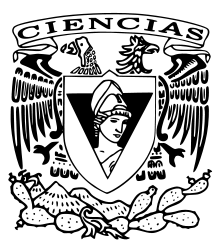
\includegraphics[scale=.29]{img/fciencias1.png}}
\end{picture}

\begin{center}
	\vspace{-114pt}
	\textbf{\large Proyecto 01}\\
	\textbf{ Semestre 2021-1}\\
	Prof. José Galaviz Casas\\
	Ayud. María Ximena Lezama \\
	\textbf{Modelado y programación}\\[0.15cm]
	Kevin Ariel Merino Peña\footnote{Número de cuenta 317031326} Armando Abraham Aquino Chapa\footnote{Número de cuenta n}
	[0.12cm]
	\today
\end{center}
\vspace{-10pt}
\rule{19cm}{0.3mm}

\begin{algorithm}
	\SetKwData{Left}{left}\SetKwData{This}{this}
	\SetKwData{Up}{up}
	\SetKwFunction{Union}{Union}
	\SetKwFunction{FindCompress}{FindCompress}
	\SetKwInOut{Input}{Entrada}
	\SetKwInOut{Output}{Salida}
	\SetAlgorithmName{Función}{0}{list of algorithms name}
	\Input{Nombre de un archivo (ruta)}
	\Output{Lista de coordenadas no repetidas}
	\BlankLine
	\While{Archivo(nombre dado) esté abierto}{
	\ForEach{renglones $\leftarrow$ documento}{
			\If{(latitud , longitud ) \textbf{no} están en  la lista}{
			Agreagrlas}
	}
}
\caption{read\_no\_repeated\_coordinates}
\end{algorithm}

\begin{algorithm}
	\SetKwData{Left}{left}\SetKwData{This}{this}
	\SetKwData{Up}{up}
	\SetKwFunction{Union}{Union}
	\SetKwFunction{FindCompress}{FindCompress}
	\SetKwInOut{Input}{Entrada}
	\SetKwInOut{Output}{Salida}
	\SetKwProg{try}{try}{:}{}
	\SetKwProg{catch}{catch}{:}{end}
	\SetAlgorithmName{Función}{0}{list of algorithms name}
	\Input{Nombre de un archivo (ruta)}
	\Output{Lista de diccionarios con vuelos}
	\BlankLine
	\try{}{
			Abrir ruta\\
			\For{linea $ \gets $ archivo}{
			linea $ \gets $ lista}
	}
	\catch{FileNotFoundError}{
		\textbf{muesta}	 Error, escribe una ruta válida\\\textbf{exit}
	}
	\catch{FileExistsError}{
	\textbf{muesta}	 Error, archivo válido\\\textbf{exit}
	}
\caption{read\_csv\_file}
\end{algorithm}

\begin{algorithm}
	\SetKwData{Left}{left}\SetKwData{This}{this}
	\SetKwData{Up}{up}
	\SetKwFunction{Union}{Union}
	\SetKwFunction{FindCompress}{FindCompress}
	\SetKwInOut{Input}{Entrada}
	\SetKwInOut{Output}{Salida}
	\SetKwProg{with}{with}{:}{}
	\SetKwProg{catch}{catch}{:}{end}
	\SetAlgorithmName{Función}{0}{list of algorithms name}
	\Input{Nombre de un archivo (ruta)}
	\Output{Lista de cabeceras}
	\BlankLine
	\with{}{
		lector $ \gets $ \textbf{Leer primera linea}( ruta)
	}
\caption{read\_headers}
\end{algorithm}
\end{document}